\documentclass[journal,12pt,onecolumn]{IEEEtran}
\usepackage[utf8]{inputenc}   % Codificación de entrada
\usepackage[T1]{fontenc}      % Codificación de fuente
\usepackage[spanish,es-tabla]{babel}   % Idioma español
\usepackage{lmodern}          % Fuente moderna
\usepackage{amsmath, amssymb} % Matemáticas y símbolos
\usepackage{graphicx} 		  % Gráficos e imágenes
\graphicspath{{img/}{tablas/}{portada/}}  % Las imágenes se buscarán en la carpeta "img"
\usepackage{longtable}      % Para tablas que se extienden en varias páginas
\usepackage{tabularx}	% Tablas avanzadas
\usepackage{threeparttable}
\usepackage{hyperref}	% Hipervínculos
\usepackage{float}
%-------------------------------------------
% Otros paquetes útiles (personaliza según tus necesidades)
%-------------------------------------------
\usepackage{caption}
\usepackage{subcaption}
\usepackage{xcolor}
\usepackage{setspace}

%-------------------------------------------
% Comandos personalizados
\renewcommand{\listtablename}{Índice de tablas}
\renewcommand{\appendixname}{Anexos}
\definecolor{colorreferences}{RGB}{48,134,3}

% Metadatos del PDF
\hypersetup{
	unicode=true,
	hidelinks,
	colorlinks=true,       % false: boxed links; true: colored links
	linkcolor=black,          % color of internal links (change box color with linkbordercolor)
	citecolor=colorreferences,        % color of links to bibliography
	filecolor=magenta,      % color of file links
	urlcolor=blue,           % color of external links
	linkbordercolor={0 0 0}
}
%-------------------------------------------
% Inicio del documento
%-------------------------------------------
\begin{document}

% Aquí se encuentra el archivo con la portada
\begin{titlepage}
	\centering
	%-------------------------------------------
	% Logos en una tabla: izquierda, centro y derecha
	\begin{tabular}{@{}p{0.3\textwidth} p{0.3\textwidth} p{0.3\textwidth}@{}}
		
\includegraphics[height=2cm]{tecnm} & 
		\centering 
\includegraphics[height=1.5cm]{SEP} & 
		\raggedleft 
\includegraphics[height=2cm]{ith.jpg} \\
	\end{tabular}
	
	\vspace{2em}
	
	\noindent
	%-------------------------------------------
	%	Información institucional y académica (esquina superior izquierda)
	\begin{minipage}[t]{0.48\textwidth}
		\raggedright
		\small \textbf{%
			Instituto Tecnológico de Hermosillo\\
			Materia: Robótica\\
			Profesor: Medina Gil Lamadrid, Jesús Iván%
		}
	\end{minipage}%
	\hfill
	%	fecha actual (esquina superior derecha), en letras pequeñas y en negrita.
	\begin{minipage}[t]{0.48\textwidth}
		\raggedleft
		\small \textbf{\today}
	\end{minipage}
	
	\vspace{2em}
	
	%-----------------------------------------
	% Unidad y Título de la tarea en letras grandes y en negrita
	{\large \textbf{Unidad 1: Morfología del robot}}\\
	{\Huge \textbf{Tipos de Sensores}}
		
	\vspace{1em}
	
	%---------------------------------------
	% Tabla con la información del equipo
	%---------------------------------------
	% Encabezado del equipo
	\begin{center}
		{\Large \textbf{Equipo 6}}
	\end{center}
	
	\vspace{1em}
	
	% Tabla de integrantes:
	% Cada fila contiene: foto (columna izquierda) y datos del integrante (columna derecha)
	\begin{center}
		\begin{tabular}{c c}
			\begin{tabular}{c}
				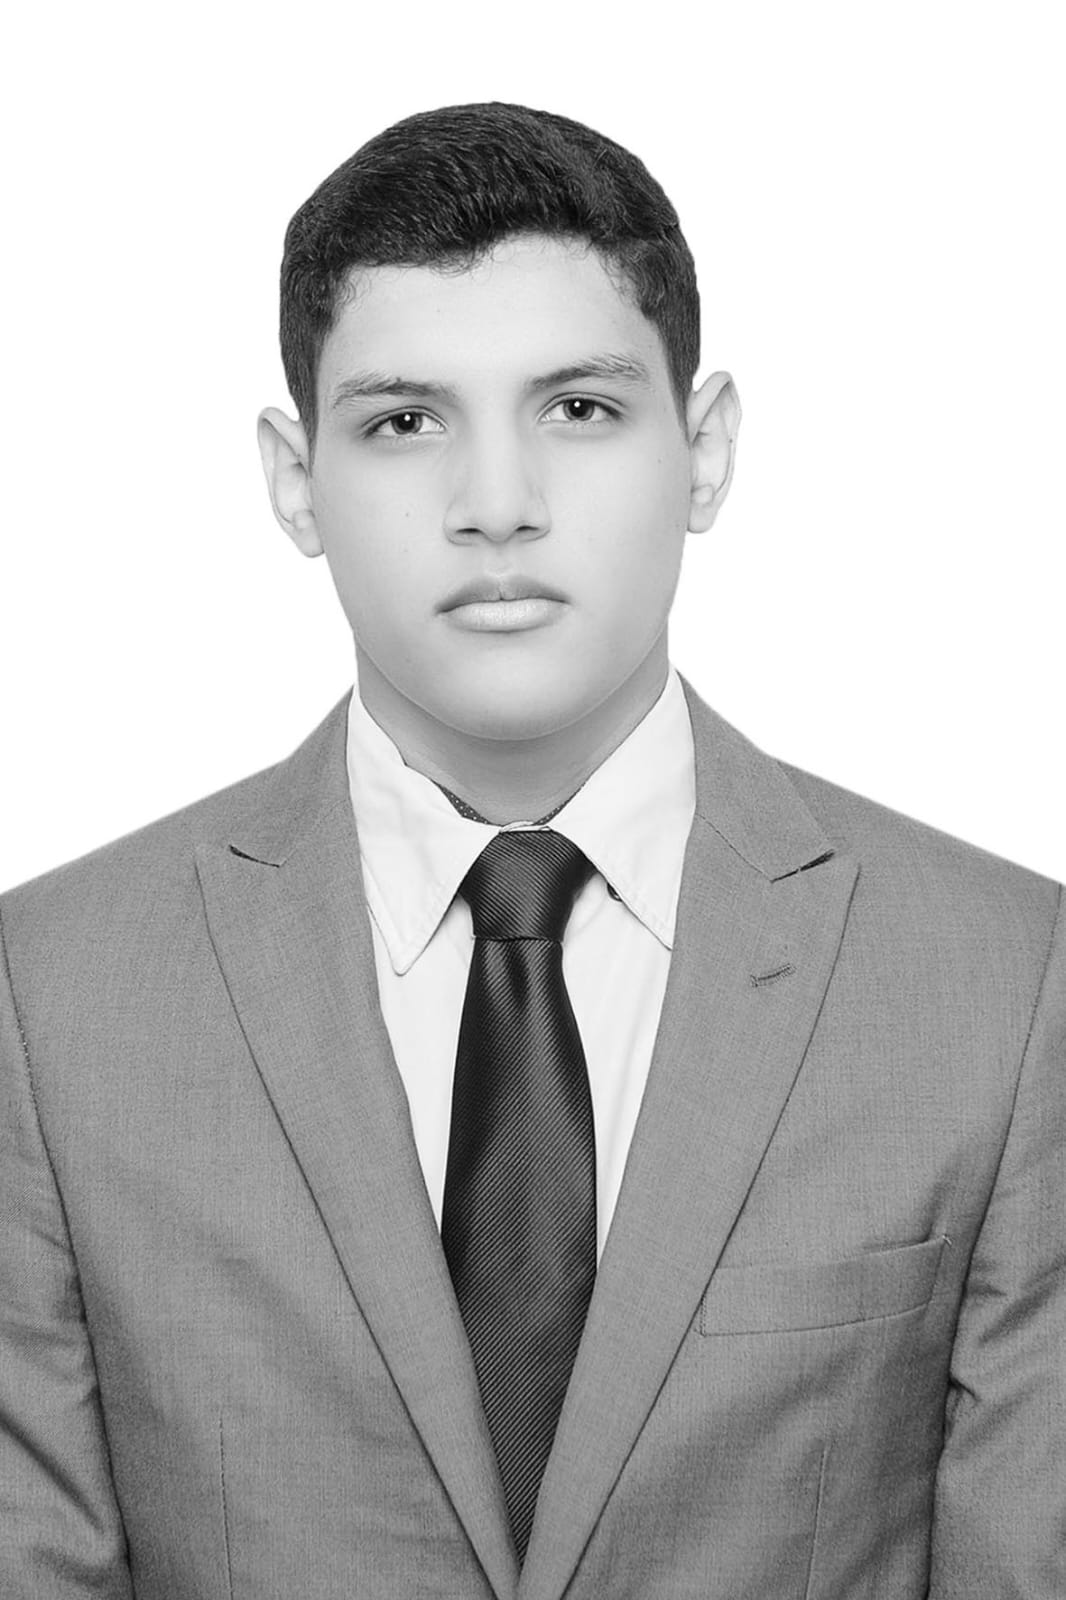
\includegraphics[height=3cm]{alexander.jpg} \\
				\textbf{Hernandez Dominguez },\\ Olinsser Alexander \\ \texttt{l21330599@hermosillo.tecnm.mx} \\ 
			\end{tabular} &
			\begin{tabular}{c}
				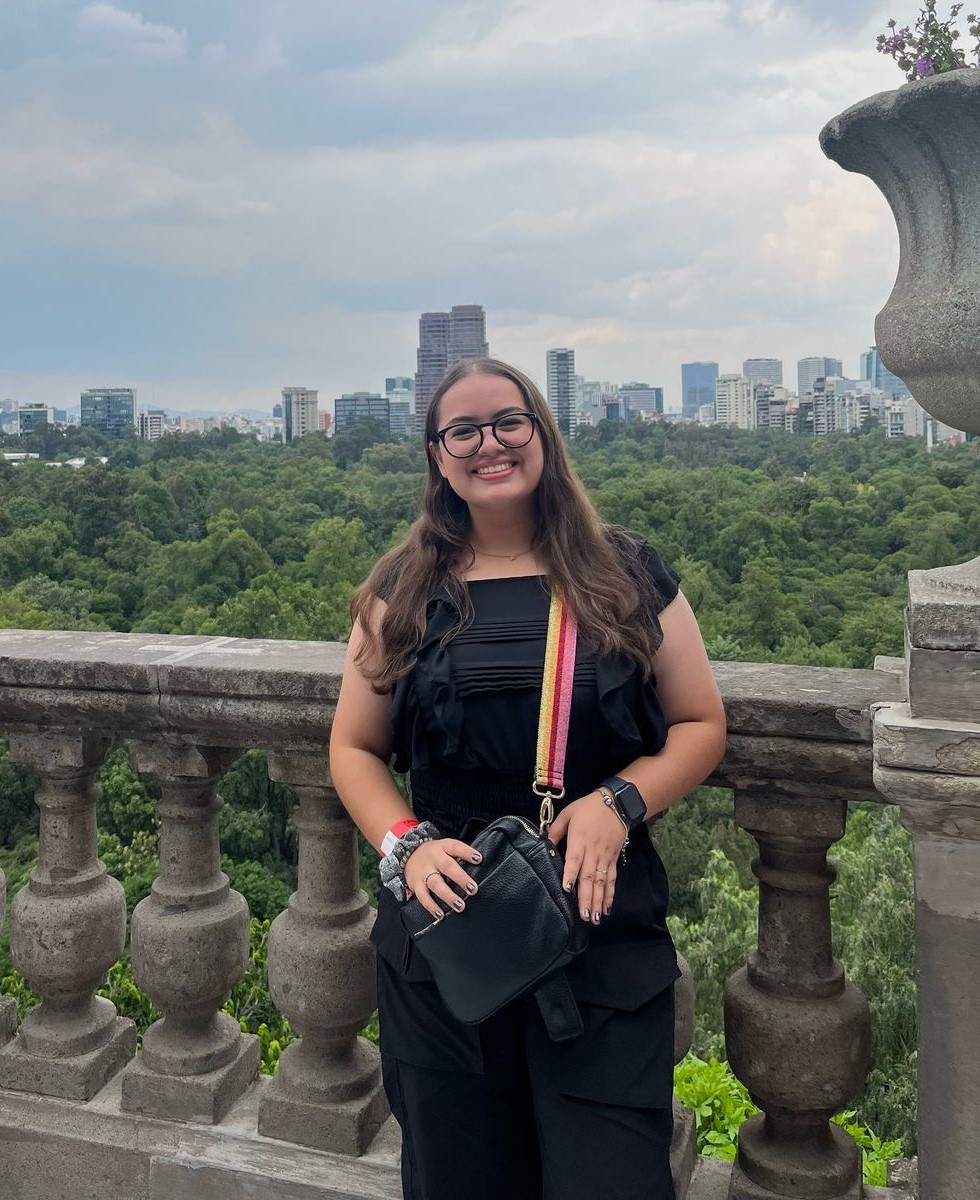
\includegraphics[height=3cm]{iliana.jpg} \\
				\textbf{Medina de la Rocha,}\\ Iliana \\ \texttt{l21330629@hermosillo.tecnm.mx} \\
			\end{tabular} \\ \vspace{2em}
			\begin{tabular}{c}
				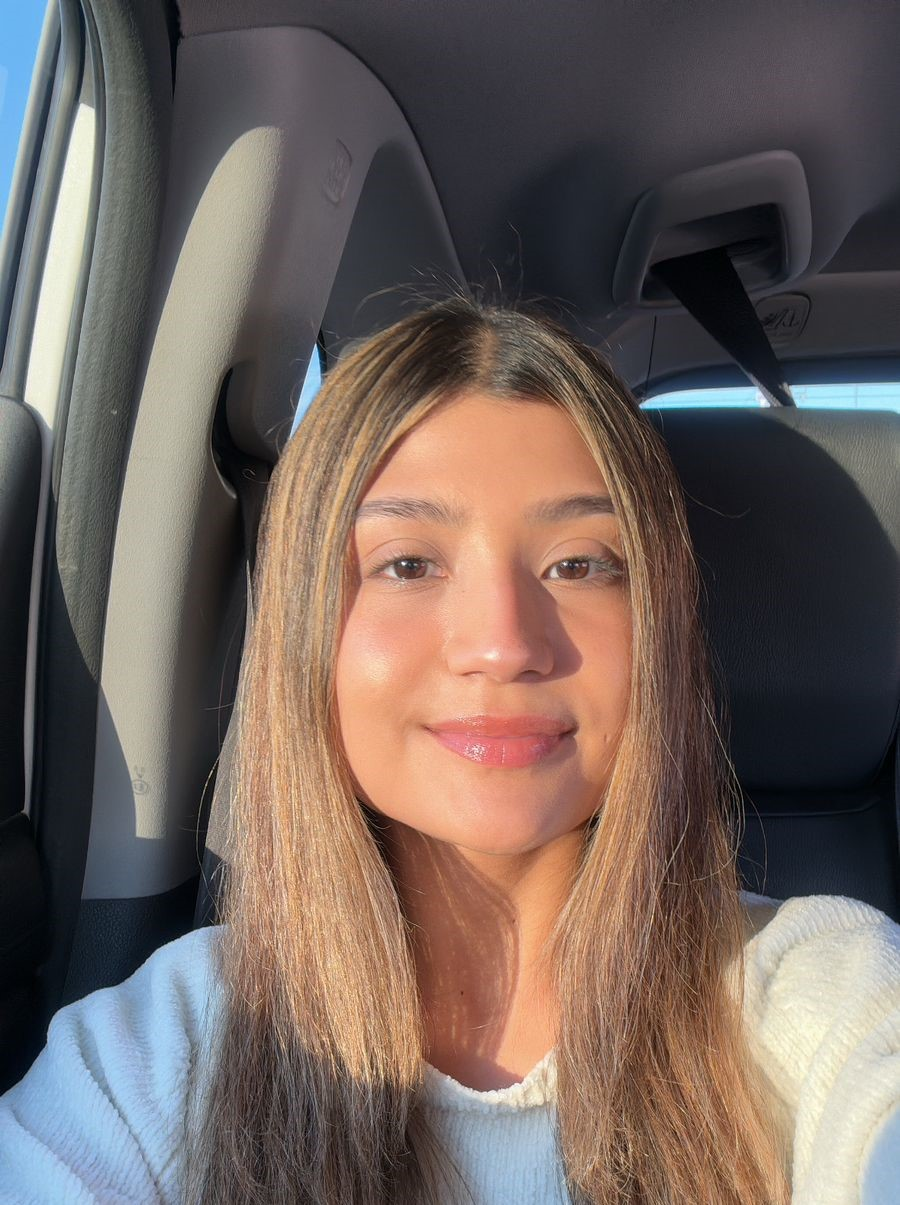
\includegraphics[height=3cm]{itzel.jpg} \\
				\textbf{Mesta Valdez,}\\ Itzel \\ \texttt{l21330635@hermosillo.tecnm.mx} \\ 
			\end{tabular} &
			\begin{tabular}{c}
				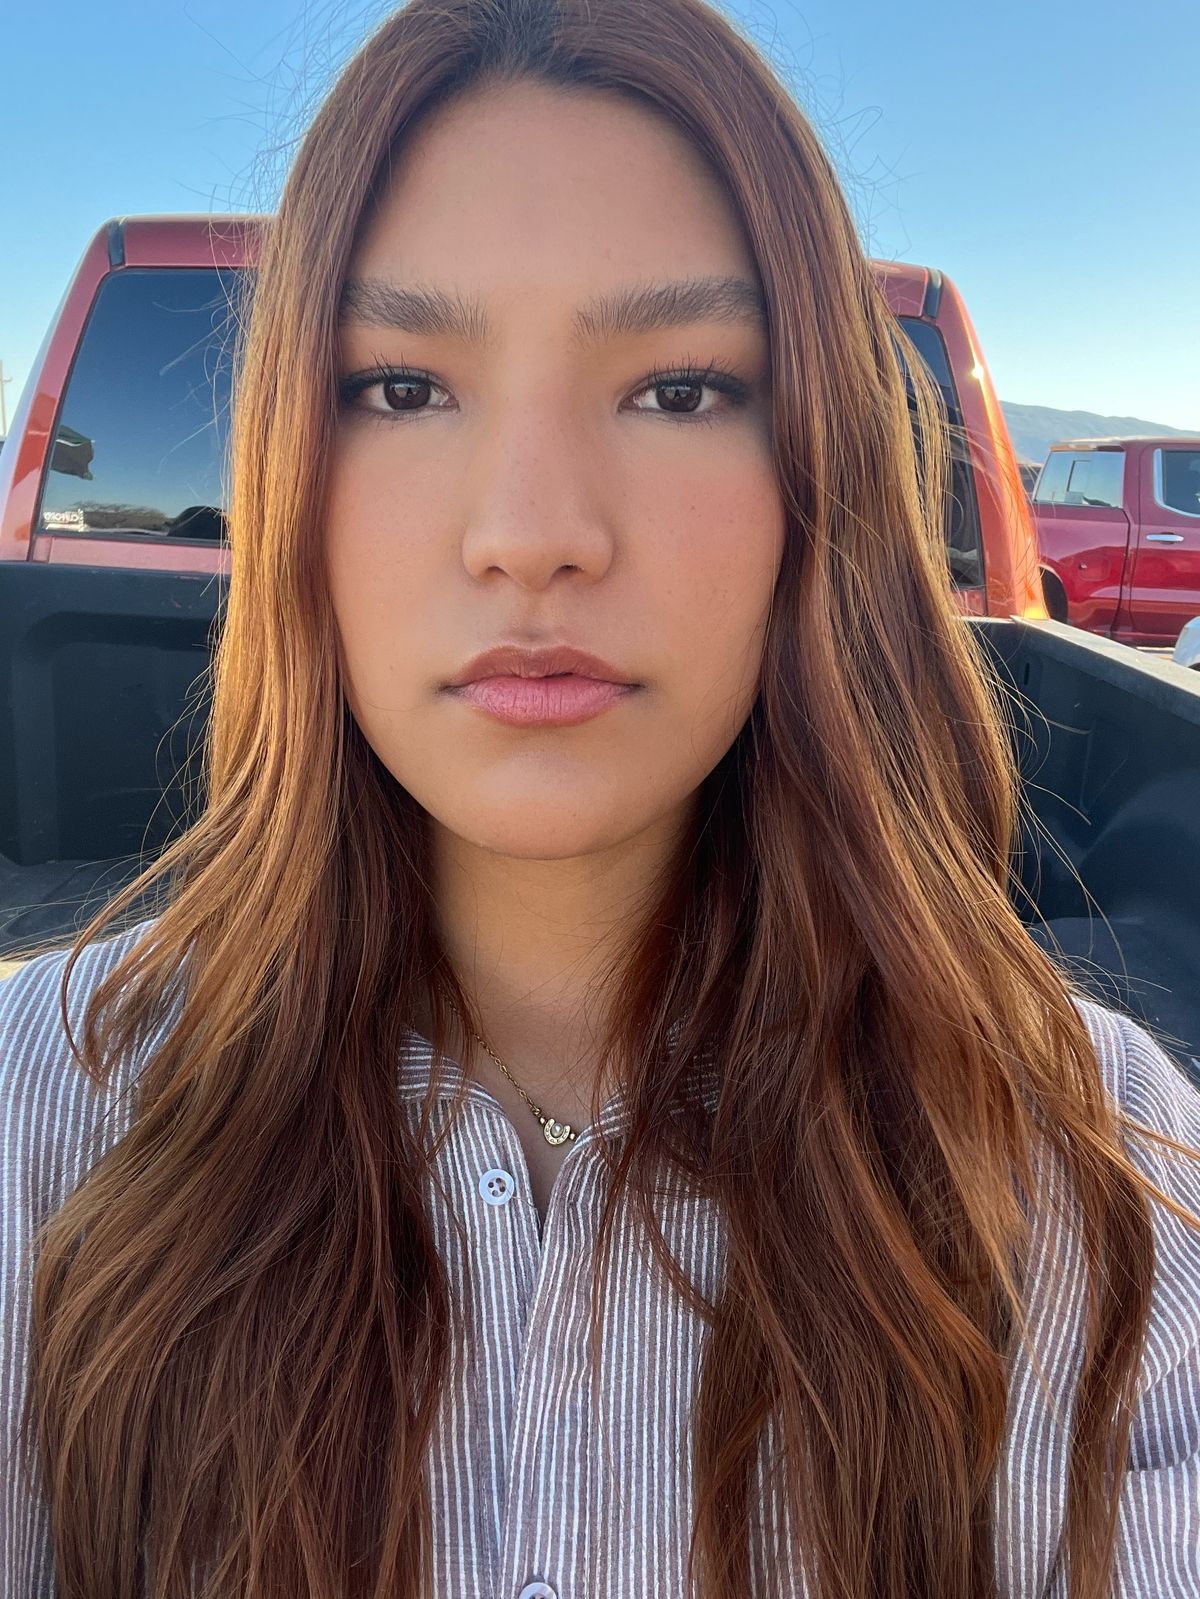
\includegraphics[height=3cm]{luisa.jpg} \\
				\textbf{Santacruz López,}\\ Luisa Fernanda \\ \texttt{l21330691@hermosillo.tecnm.mx} \\ 
			\end{tabular}
		\end{tabular}
	\end{center}

\end{titlepage}

%	Es innecesario poner el índice porque ya aparece en los marcadores del PDF
%\tableofcontents

% Ejemplo de inclusión de una sección (por ejemplo, "introduccion.tex" debe estar en la carpeta "secciones" y se recomienda no usar carácteres especiales (tilde) o espacios)
\section{Ejercicios Denavit Hartenberg}

El presente documento contiene el desarrollo de ejercicios enfocados en la cinemática inversa de dos robots diferentes al robot 1, conforme a las indicaciones establecidas en la tarea. Cada robot fue programado y simulado utilizando MATLAB, generando animaciones que muestran el movimiento del robot al alcanzar un objetivo específico en el espacio.

La cinemática inversa permite determinar los ángulos articulares necesarios para que el efector final del robot alcance una posición deseada. En este reporte se presentan los resultados obtenidos para cada uno de los robots seleccionados, así como las gráficas correspondientes a su trayectoria.

Además, se calcula y analiza el error del objetivo alcanzado, con el fin de evaluar la precisión de cada solución obtenida. Los videos generados durante la simulación han sido guardados y, junto con los archivos de código, pueden encontrarse en el repositorio correspondiente o se adjuntan a este reporte según lo solicitado.
	\subsection{Sensores de Posición}
\subsubsection{Lineales y Rotativos}
Los sensores de posición lineal incluyen:

\begin{itemize}
	\item \textbf{Encóder incremental}:Este tipo de sensor convierte el movimiento en una serie de pulsos eléctricos que indican cambios en la posición, pero no su valor absoluto. Requiere un punto de referencia para determinar la posición inicial y utiliza dos señales desfasadas (A y B) para detectar dirección y velocidad. Estos constan, en su forma más simple, de un
	disco transparente con una serie de marcas opacas colocadas radialmente y equidistantes entre sí; de un sistema de iluminación en el que la luz es colimada de forma correcta, y de un elemento fotorreceptor (Figura 1). El eje, cuya posición se quiere medir, va acoplado al disco transparente. Con esta disposición, a medida que el eje gire se irán generando pulsos en el receptor cada vez que la luz atraviese cada marca. Llevando una cuenta de estos pulsos será posible conocer la posición del eje.
	\begin{figure}[h]
		\centering
		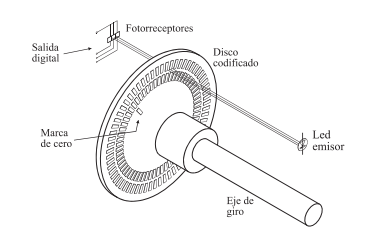
\includegraphics[width=0.8\textwidth]{img/encoderincremental.png}
		\caption{Disposición de un codificador óptico (encóder) incremental.}
		\label{fig:encoderincremental}
	\end{figure}
	
	
	\item \textbf{Encóder absoluto}:A diferencia del incremental, el encoder absoluto proporciona la posición exacta en todo momento, incluso después de un apagado. Funciona mediante un disco codificado con un patrón único para cada posición, permitiendo lecturas precisas sin necesidad de reiniciar.
	\begin{figure}[h]
		\centering
		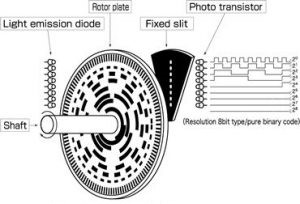
\includegraphics[width=0.6\textwidth]{img/encoderabsoluto.jpg}
		\caption{Estructura simplificada del encóder absoluto.}
		\label{fig:encoderabsoluto}
	\end{figure}
	
	
	\item \textbf{Potenciómetro}: Es un dispositivo de resistencia variable que expresa desplazamientos lineales o angulares en términos de voltaje, tal como se muestra en las figuras 3a) y b), respectivamente. Consiste en una clavija deslizante que hace contacto con un elemento resistivo; conforme se mueve este punto de contacto, la resistencia entre el contacto deslizante y las conexiones de los extremos del dispositivo cambia en proporción al desplazamiento, x y  para potenciómetros lineales y angulares, respectivamente.
	\begin{figure}[h]
		\centering
		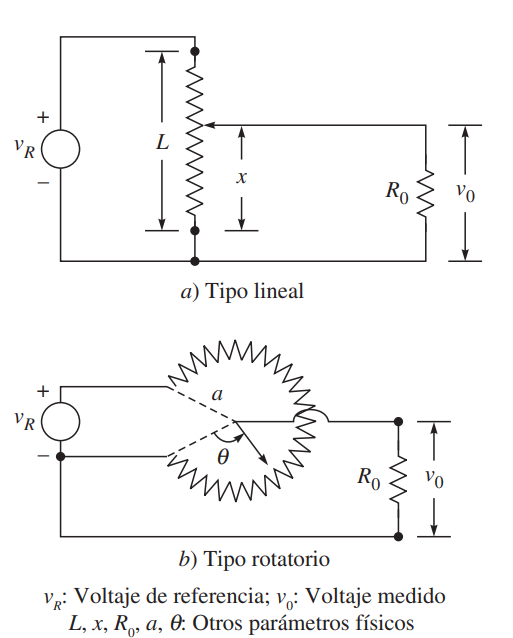
\includegraphics[width=0.4\textwidth]{img/potenciometro.png}
		\caption{Potenciómetros.}
		\label{fig:potenciometros}
	\end{figure}
	
	
	
	\item \textbf{LVDT}: El transformador diferencial lineal variable (LVDT) es un sensor de desplazamiento altamente preciso y confiable. Funciona con una señal de corriente alterna (CA), generando un voltaje proporcional al desplazamiento del núcleo móvil dentro de un campo magnético. Su estructura incluye un núcleo central rodeado por bobinas secundarias y una bobina primaria que crea el campo magnético. A medida que el núcleo se mueve, la señal de salida cambia de manera lineal con el desplazamiento. También existe el transformador diferencial rotativo (RVDT), que opera con el mismo principio pero para movimientos angulares. Su principio de funcionamiento es basado en la inducción electromagnética. En el esquema de la Figura 4, se observa un núcleo ferromagnético móvil que se desplaza dentro de un conjunto de bobinas:
	\item \textbf{Bobina primaria (Lp)}: Recibe una señal de excitación en corriente alterna (CA) y genera un campo magnético.
	\item \textbf{Bobinas secundarias (Ls1 y Ls2)}: Están ubicadas a ambos lados del núcleo y captan la variación del flujo magnético cuando el núcleo se mueve.
	\item \textbf{Núcleo móvil}: se mueve dentro de las bobinas y altera la relación de inductancias.
	
	El desplazamiento del núcleo altera la relación de inductancias entre las bobinas secundarias, modificando así la amplitud y fase de la señal de salida. Esto permite determinar la posición del núcleo con alta precisión.
	
	Si el núcleo está en el centro, las señales en las bobinas secundarias son iguales y opuestas, generando una salida cero. Cuando el núcleo se desplaza, una de las bobinas capta más flujo que la otra, lo que genera un voltaje proporcional al movimiento.
	\begin{figure}[h]
		\centering
		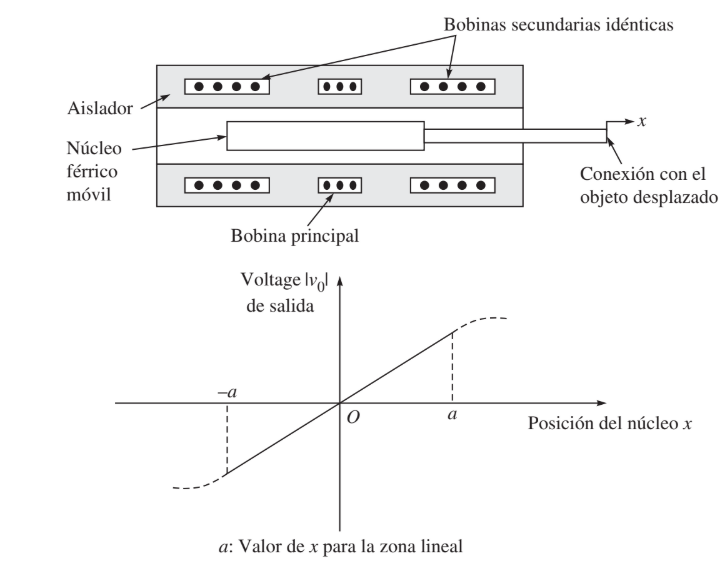
\includegraphics[width=0.700\textwidth]{img/lvdt.png}
		\caption{Esquema de funcionamiento de un LVDT.}
		\label{fig:lvdt}
	\end{figure}
	
	
	\item \textbf{Résolver}: Los resólvers proporcionan señales análogas como salida. Éstos consisten en un eje (flecha) giratorio (rotor) y una carcasa estacionaria (estator). Sus señales tienen que convertirse a la forma digital por medio de un convertidor analógico a digital antes de que la señal sea introducida a la computadora.Su funcionamiento se basa en la conversión de la posición angular del rotor en señales eléctricas proporcionales al ángulo de giro.
	
	Los resolvers se utilizan para medir el ángulo de un eje en aplicaciones donde los encoders no son viables debido a condiciones extremas como temperatura, vibraciones o interferencias electromagnéticas. Funcionan aplicando una señal de referencia de corriente alterna (CA) al rotor, lo que induce tensiones en las bobinas del estator dispuestas a 90° entre sí. Estas señales de salida tienen amplitudes proporcionales al seno y coseno del ángulo del rotor, lo que permite determinar la posición angular con alta precisión.
	\begin{figure}[h]
		\centering
		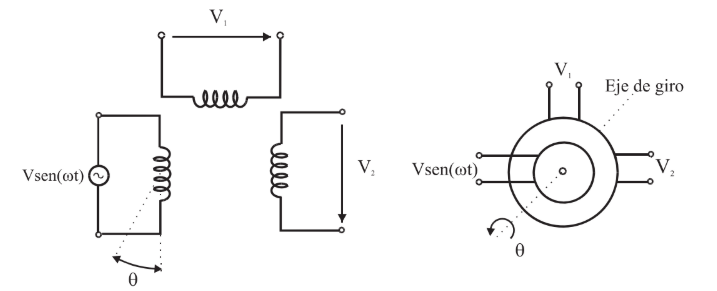
\includegraphics[width=\textwidth]{img/resolver.png}
		\caption{Esquema de funcionamiento de un resolver.}
	\end{figure}
	
	
	La imagen Figura 5 muestra el esquema de funcionamiento de un resolver, un sensor electromecánico utilizado para medir la posición angular de un eje. En el diagrama se observa un rotor, que es la parte móvil del dispositivo y está conectado al eje de giro, y un estator, que es la parte fija y contiene dos bobinas ubicadas en cuadratura, es decir, dispuestas a 90° entre sí. La señal de referencia, representada como V\( _{\text{sen}}(\omega t) \), se aplica a la bobina del rotor, lo que genera un acoplamiento electromagnético con las bobinas del estator. Este acoplamiento hace que las bobinas del estator induzcan voltajes proporcionales al ángulo $\theta$ del rotor.
	Las ecuaciones que describen el comportamiento del resolver son:
	
	\begin{equation}
		V_1 = V \sin(\omega t) \sin(\theta)
	\end{equation}
	
	\begin{equation}
		V_2 = V \sin(\omega t) \cos(\theta)
	\end{equation}
	
	Esto significa que la señal de salida en el estator depende del seno y el coseno del ángulo de giro del rotor, lo que permite calcular con precisión su posición angular mediante la relación entre ambas tensiones.  
	
\end{itemize}

\subsection{Sensores de Velocidad}
La captación de la velocidad se hace necesaria para mejorar el comportamiento dinámico de
los actuadores del robot. La velocidad de movimiento de cada actuador (que tras el reductores la velocidad de la articulación) se realimenta normalmente a un bucle de control analógico implementado en el propio accionador del elemento motor. No obstante, en ocasiones en las que el sistema de control del robot lo exija, la velocidad de giro de cada actuador es llevada hasta la unidad de control del robot.

Los sensores de velocidad incluyen:

\begin{itemize}
	\item \textbf{Todos los sensores de posición}
	\item \textbf{Tacómetro}: Estos sensores pueden encontrar directamente la velocidad en cualquier momento y sin mucha carga computacional. Éstos miden la velocidad de rotación de un elemento. Hay varios tipos de tacómetros en uso, pero un diseño sencillo se basa en la regla de Fleming, que declara que “el voltaje producido es proporcional al índice del acoplamiento inductivo”. Aquí un conductor (básicamente una bobina) se sujeta al elemento rotativo que gira en un campo magnético (estator). Conforme incrementa la velocidad del eje, el voltaje producido en las terminales de las bobinas también aumenta. De otra manera, como se muestra en la figura 6, puede colocarse un imán sobre el eje rotativo y una bobina sobre el estator. El voltaje producido es proporcional a la velocidad de rotación del eje. Esta información se digitaliza mediante un convertidor analógico-digital y se introduce en la computadora.
	\begin{figure}[h]
		\centering
		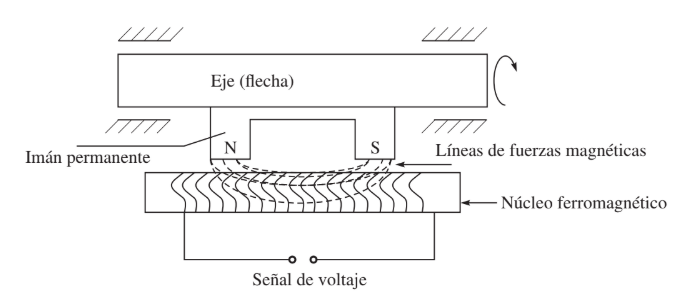
\includegraphics[width=\textwidth]{img/Diagramatacometro.png}
		\caption{Diagrama Tacómetro}
	\end{figure}
	
	
	\item \textbf{Sensor de efecto Hall}: El  principio de este sensor es el siguiente: Si una pieza plana de material conductivo llamada chip Hall se sujeta a una diferencia de potencial en sus dos lados opuestos como se indica en la figura 7, entonces el voltaje que se genera a través de las caras perpendiculares es cero. Pero si un campo magnético se induce en ángulos rectos al conductor, el voltaje se genera en las otras dos caras perpendiculares. Entre más alto sea el valor de campo, más lo será el nivel de voltaje. Si se utiliza un imán anular, el voltaje producido será proporcional a la velocidad de rotación del imán. 
	\begin{figure}[h]
		\centering
		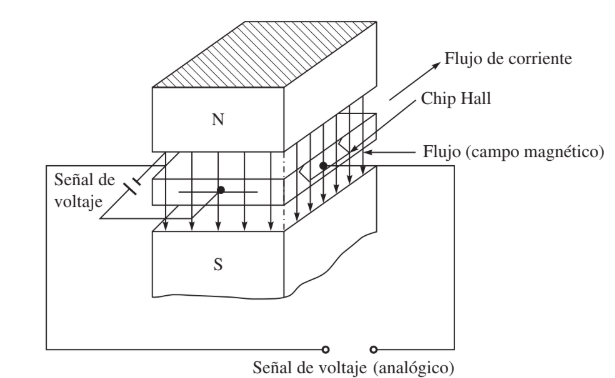
\includegraphics[width=\textwidth]{img/sensorhall.png}
		\caption{Sensor Hall}
	\end{figure}
	
\end{itemize}

\subsection{Sensores de Aceleración}
La aceleración puede obtenerse a partir de los sensores de velocidad o calculando el cambio en la posición, pero este método es ineficiente y sobrecarga la computadora, afectando el rendimiento del sistema. Una alternativa es medirla mediante la fuerza, aplicando la fórmula masa por aceleración. 
Las fuerzas se miden usando la fórmula de las galgas extensométricas, mediante la relación \( F = \frac{\Delta RAE}{RC} \) y dividiéndola por la masa del objeto obtenemos la formula de la aceleración: \[a = \frac{\Delta R A E}{R C m} \]. Donde: \begin{itemize}
	\item $F$: fuerza
	\item $\Delta R$: cambio de resistencia de la galga
	\item $A$: área
	\item $E$: módulo de elasticidad del material de la galga
	\item $R$: resistencia original de la galga
	\item $C$: constante de deformación de la galga
\end{itemize}
Este método es preferible, ya que evita la amplificación del ruido que ocurre al calcular la aceleración desde la velocidad, donde se requiere diferenciación. En cambio, la integración de la fuerza ayuda a suprimir el ruido en la señal.
Los sensores de aceleración incluyen:
\begin{itemize}
	\item \textbf{Todos los sensores de fuerza}
\end{itemize}
\subsection{Sensores de Fuerza}	
\begin{itemize}
	\item \textbf{Galgas extensométricas}: Este sensor interno tiene como principio que: “el alargamiento de un conductor aumenta su resistencia eléctrica”, debido a 2 razones principales:
	
	-	Incremento de la longitud del conductor.
	
	-	Decremento en el área del conductor.
	
	
	
	De esta forma, se pueden detectar las variaciones, ya que una resistencia normal para galgas es de 50 a 100 ohmios.
	
	Cuando el objeto al que está adherida la galga se deforma (por tensión o compresión), la longitud y la sección transversal del material de la galga cambian, lo que modifica su resistencia eléctrica. Esta variación de resistencia se mide con un circuito en puente de Wheatstone y se convierte en una señal eléctrica proporcional a la deformación.
	\begin{figure}[h]
		\centering
		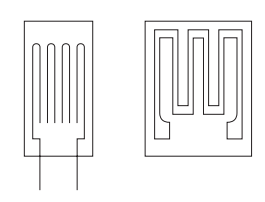
\includegraphics[width=0.5\textwidth]{img/galgas.png}
		\caption{Galgas extensométricas}
	\end{figure}
	
	\item \textbf{Interruptores de efecto Hall}: Los interruptores de efecto Hall son sensores electrónicos que detectan la presencia de un campo magnético y generan una señal de salida en respuesta.
	
	Cuando un material conductor o semiconductor, como el silicio, se somete a un campo magnético perpendicular a la dirección de la corriente que circula a través de él, se genera una diferencia de potencial (voltaje Hall) en dirección perpendicular a ambos.
	
	Los interruptores de efecto Hall utilizan este principio para detectar campos magnéticos y generar una señal de encendido o apagado.
	\begin{figure}[h]
		\centering
		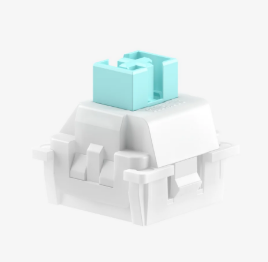
\includegraphics[width=0.5\textwidth]{img/interruptorhall.png}
		\caption{Interruptor de efecto Hall}
	\end{figure}
	
	
	\item \textbf{Interruptores piezoeléctricos}: Este sub tipo de sensor interno de fuerza utiliza el principio del efecto piezoeléctrico, el cual señala que: “cuando cristales elásticos asimétricos se deforman mediante una fuerza, se desarrollará un potencial eléctrico dentro de la red cristalina deformada”.
	
	Cuando se aplica una presión sobre la superficie del interruptor, el material piezoeléctrico dentro del dispositivo genera una pequeña carga eléctrica. Esta señal es procesada y utilizada para activar o desactivar un circuito, funcionando como un interruptor táctil sin desgaste mecánico.
	\begin{figure}[h]
		\centering
		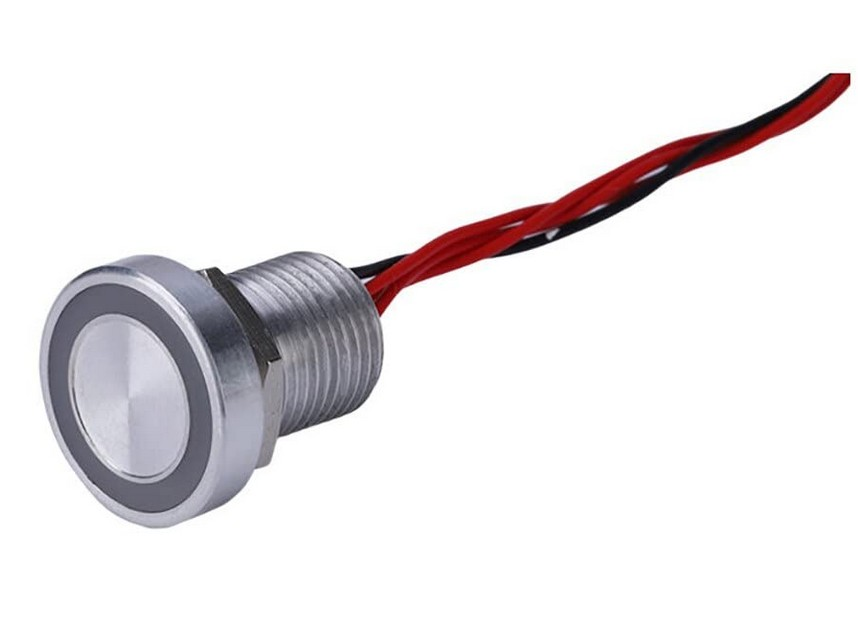
\includegraphics[width=0.5\textwidth]{img/piezoelectric-switch.jpg}
		\caption{Interruptor piezoeeléctrico}
	\end{figure}
	
\end{itemize}

	\subsection{Sensores de Contacto}
\section{Sensores Externos}
\begin{itemize}
	\item \textbf{Interruptores de límite}: El interruptor de límite es un sensor mecánico que se activa al ser presionado, generalmente mediante un brazo mecánico, y puede operar con contacto directo o mediante un imán. Existen en configuraciones normalmente abiertas (NO) y normalmente cerradas (NC), permitiendo o interrumpiendo el flujo de corriente según su activación. También pueden tener uno o varios polos para controlar distintos circuitos. Aunque son fiables, presentan desventajas como desgaste mecánico y menor velocidad en comparación con sensores sin contacto. Se utilizan en robots para detectar posiciones extremas y detener actuadores, evitando daños en la estructura mecánica.
	\begin{figure}[H]
		\centering
		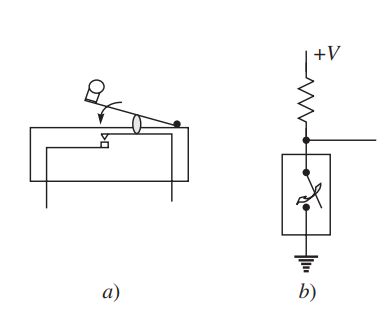
\includegraphics[width=0.5\textwidth]{interruptordelim.png}
		\caption{Interruptor de límite}
	\end{figure}
	
	\item \textbf{Interruptores neumáticos}:Un interruptor neumático es un tipo de dispositivo de conmutación que utiliza aire para funcionar. Cuando se comprime, el interruptor neumático envía un soplo o una bocanada de aire a lo largo de un tubo de PVC hasta un interruptor de aire. El movimiento del aire activará el interruptor de aire, que creará el circuito eléctrico y activará un dispositivo. Los interruptores neumáticos son muy populares y forman parte de nuestra cartera de productos. Debido a que los interruptores neumáticos son necesarios en muchas aplicaciones e industrias.
	\begin{figure}[H]
		\centering
		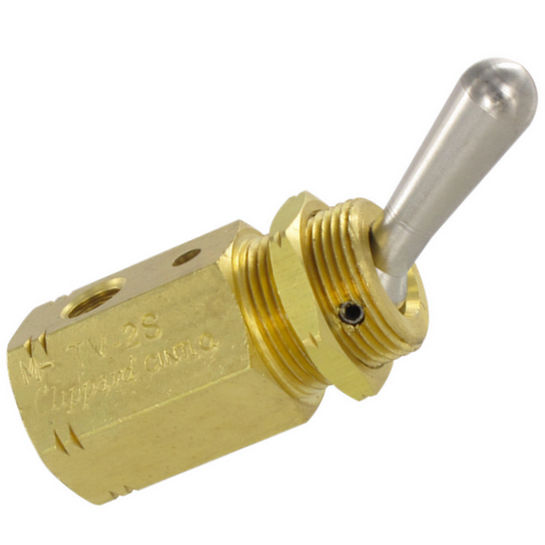
\includegraphics[width=0.35\textwidth]{interruptorneumatico.jpg}
		\caption{Interruptor neumático}
	\end{figure}
	
	
	\item \textbf{Sensores piezoeléctricos}:Un sensor piezoeléctrico es un dispositivo basado en la teoría del efecto piezoeléctrico, el cual es utilizado para medir presión, aceleración, tensión o fuerza; transformando las lecturas en señales eléctricas. Para obtener propiedades piezoeléctricas, el material debe someterse a un fuerte campo eléctrico para secuenciar las cargas. Siendo eliminado el campo eléctrico, la carga se liberará y cuando se aplique presión, la carga se reorganizará para provocar la carga deseada. 
	\begin{figure}[H]
		\centering
		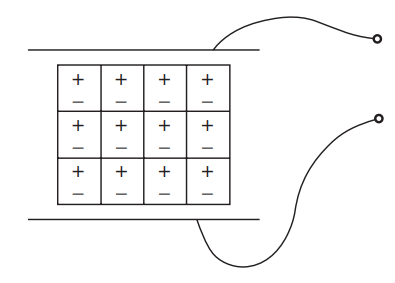
\includegraphics[width=0.5\textwidth]{sensorpiezoelectrico.png}
		\caption{Sensor Piezoeléctrico}
	\end{figure}
	
	\item \textbf{Transductores de presión}:Un transductor de presión convierte la presión en una señal de salida eléctrica. La señal eléctrica puede ser digital o analógica y es utilizada por otros dispositivos como controladores, alarmas y otros sistemas de circuito cerrado. Los transductores de presión se utilizan ampliamente en diversas aplicaciones residenciales y comerciales como bombas, vehículos, aeronaves, etc., donde se requiere la medición de presión. Estos dispositivos son cruciales para garantizar la seguridad y eficiencia en los sistemas al proporcionar datos de presión precisos y en tiempo real.
\end{itemize}
\begin{figure}[H]
	\centering
	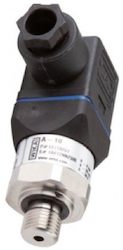
\includegraphics[width=0.125\textwidth]{pressure-transducer.png}
	\caption{Transductor de presión}
\end{figure}

\subsection{Sensores sin Contacto}
\begin{itemize}
	\item \textbf{Sensores de proximidad}: Los sensores de proximidad permiten detectar la presencia o ausencia de objetos sin contacto físico. Se dividen en inductivos y capacitivos.
	\subitem \textbf{ 1.Sensor de proximidad inductivo}: Diseñado para detectar objetos metálicos mediante un campo magnético generado
	por un oscilador.
	\subsubitem -Compuesto por cuatro elementos: bobina y núcleo férrico, circuito oscilador, circuito
	detector y circuito de salida de estado sólido.
	\subsubitem -Funciona detectando cambios en la amplitud del oscilador cuando un objeto entra o
	sale del campo magnético.
	\subsubitem -Tiene un rango de detección típico de 10-15 mm, aunque algunos alcanzan hasta
	100 mm.
	\subsubitem -Factores mecánicos y ambientales pueden afectar su precisión.
	\begin{figure}[H]
		\centering
		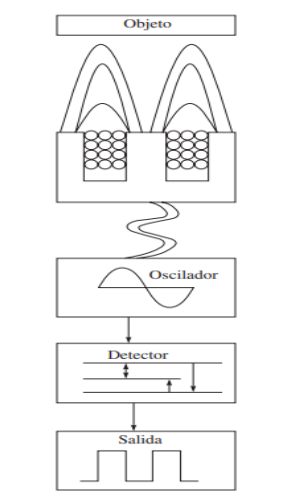
\includegraphics[width=0.3\textwidth]{sensorproxin.png}
		\caption{Sensor de proximidad inductivo} 
	\end{figure}
	\subitem \textbf{ 2.Sensor de proximidad capacitivo}: Similar al inductivo, pero funciona con la capacitancia dieléctrica, permitiendo detectar tanto objetos metálicos como no metálicos.
	\subsubitem -Compuesto por los mismos cuatro elementos del sensor inductivo.
	\subsubitem -Puede detectar objetos ligeros, pequeños y a través de barreras no metálicas (vidrio,plástico).
	\subsubitem - Presenta ventajas como alta velocidad de conmutación, larga vida útil y señal sin rebotes.
	\subsubitem -Limitaciones: afectado por humedad y vaho, y requiere un ajuste de sensibilidad
	para optimizar su rango de detección.
	\subsubitem -Posee mayor alcance que los sensores inductivos y su detección depende del área del plato sensor.
	
	Estos sensores se utilizan ampliamente en la automatización industrial para detectar objetos
	sin contacto, mejorando la eficiencia y precisión en diversas aplicaciones.
	\begin{figure}[H]
		\centering
		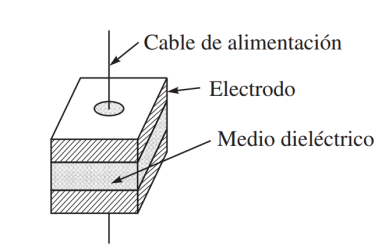
\includegraphics[width=0.4\textwidth]{sensorproxcap.png}
		\caption{Sensor de proximidad capacitivo} 
	\end{figure}
	\item \textbf{Sensores de efecto Hall}: El sensor de efecto Hall es un dispositivo electrónico utilizado para medir campos magnéticos, aprovechando el fenómeno físico conocido como el efecto Hall. Este sensor detecta la presencia, intensidad y dirección de un campo magnético, generando una señal de salida proporcional a la variación del campo. Los sensores de efecto Hall se utilizan principalmente para aplicaciones de posicionamiento, velocidad y control de motores, al detectar la posición de un imán o la rotación de ejes. Son muy útiles en sistemas de retroalimentación, ya que proporcionan una medición precisa sin contacto directo, lo que los hace ideales para entornos en los que se requiere alta fiabilidad y durabilidad. Además, su
	capacidad para operar en condiciones difíciles, como altas temperaturas o ambientes polvorientos, los convierte en una opción valiosa en la automatización y control robótico. 
	\begin{figure}[H]
		\centering
		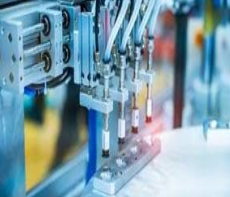
\includegraphics[width=0.4\textwidth]{sensorhallsc.png}
		\caption{Sensor de efecto Hall} 
	\end{figure}
	Ofrecen varias ventajas, como su inmunidad al ruido eléctrico y al polvo, su fiabilidad debido a la ausencia de partes móviles, y su durabilidad gracias a su diseño en estado sólido. Además, son capaces de funcionar en condiciones extremas, sin sufrir rebotes de contacto, lo que les proporciona una larga vida útil. Estos sensores se aplican en áreas como servomotores, sensores de proximidad y velocidad, sistemas de inyección automovilísticos, control de acceso y medición de potencia y campo magnético, siendo esenciales en la
	automatización industrial y el control de movimiento.
	\begin{figure}[H]
		\centering
		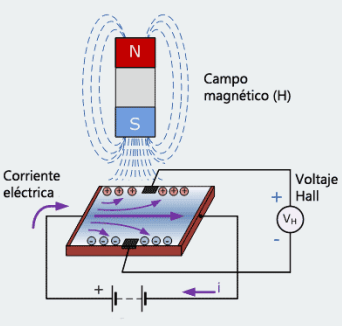
\includegraphics[width=0.4\textwidth]{sefectohall.png}
		\caption{Principios básicos de los sensores de efecto Hall} 
	\end{figure}
	
	\item \textbf{Sensores de microondas}: Los sensores de microondas emplean la frecuencia de microondas para detectar movimiento mediante la emisión de impulsos y el análisis de su reflejo en objetos en movimiento, basándose en el efecto Doppler.
	\begin{figure}[H]
		\centering
		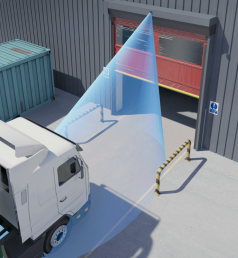
\includegraphics[width=0.4\textwidth]{sensormicroondas.png}
		\caption{Sensor de microondas} 
	\end{figure}
	
	\subitem \textbf{Tipos de Sensores de Microondas}:
	\subsubitem 	1. Radar de Onda Continua (CW): Emite señales continuas y detecta cambios en el
	patrón de reflexión para identificar movimiento.
	\subsubitem 2. Radar de Impulsos: Envía impulsos de microondas y mide el tiempo de retorno para
	determinar la distancia del objeto.
	\subsubitem 3. Radar Doppler: Mide el cambio en la frecuencia de la onda reflejada para detectar
	movimiento.
	\subsubitem 	4. Sensores Biestáticos: Separan la unidad emisora y la receptora, mejorando la
	precisión y reduciendo falsas alarmas.
	\subsubitem 5. Sensores Monostáticos: Integran emisor y receptor en una sola unidad, ofreciendo
	mayor compactación.
	
	Los sensores de microondas son fundamentales en la seguridad perimetral debido a su
	amplia cobertura, lo que los hace ideales para proteger grandes áreas como aeropuertos y
	bases militares. Son efectivos en la reducción de falsas alarmas al diferenciar entre intrusos
	humanos y movimientos de animales o vegetación. Además, funcionan en condiciones
	climáticas adversas como lluvia, niebla o nieve, y se integran con sistemas de CCTV para
	activar grabaciones ante detección de movimiento. Su diseño discreto dificulta su evasión
	por parte de intrusos, y su versatilidad permite combinarlos con otros sistemas de
	seguridad, ofreciendo una protección confiable y efectiva.
	\begin{figure}[H]
		\centering
		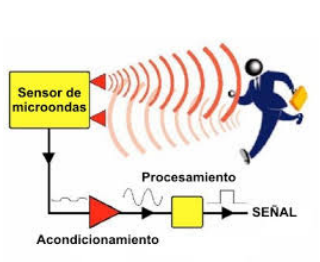
\includegraphics[width=0.4\textwidth]{sensormicro.png}
		\caption{Principios básico de sensores de microondas} 
	\end{figure}
	
	
	
	\item \textbf{Sensores ultrasónicos}: Los sensores ultrasónicos son dispositivos avanzados que utilizan ondas sonoras de alta	frecuencia para detectar objetos y medir distancias con gran precisión. Su función es
	esencial en la robótica, ya que permiten que las máquinas perciban su entorno, facilitando
	una detección confiable y precisa de obstáculos.
	
	La capacidad de detección y evitación de objetos es crucial para la navegación y operación
	eficiente de los robots, especialmente en aplicaciones críticas como vehículos autónomos y
	robots médicos. Sin estos sistemas, los robots podrían enfrentar dificultades para reconocer
	su entorno, lo que podría generar accidentes o fallos en su desempeño. Para mejorar estas
	capacidades, los ingenieros emplean tecnologías avanzadas como visión por computadora,
	aprendizaje automático y sensores ultrasónicos, optimizando así la seguridad, eficiencia y
	automatización en diversas industrias. Los sensores ultrasónicos, como el HC-SR04,
	funcionan emitiendo ondas sonoras de alta frecuencia que rebotan en los objetos,
	permitiendo calcular con precisión la distancia. Son especialmente útiles en entornos
	desafiantes, como áreas con polvo o humo, donde otros sensores pueden fallar. Sin
	embargo, pueden experimentar interferencias, que se resuelven mediante técnicas como el
	salto de frecuencia.
	\begin{figure}[H]
		\centering
		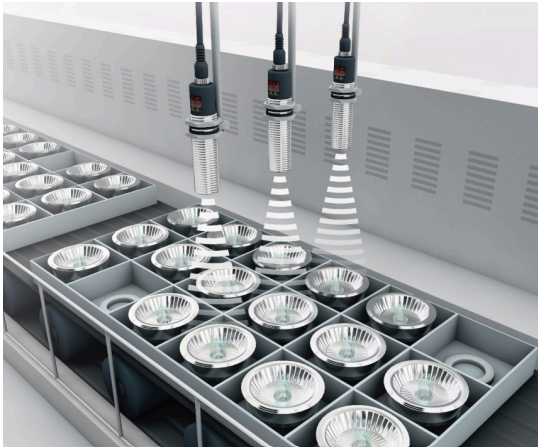
\includegraphics[width=0.4\textwidth]{sultra.png}
		\caption{Sensor Ultrasónico} 
	\end{figure}
	Cálculo de distancia con sensores ultrasónicos:
	
	El sensor ultrasónico mide la distancia de un objeto mediante la siguiente fórmula:
	
	Distancia = (Tiempo de eco x Velocidad del sonido en el aire) / 2
	
	Este método garantiza mediciones exactas y es especialmente útil en entornos donde otros
	sensores, como los infrarrojos, pueden no ser efectivos.
	\begin{figure}[H]
		\centering
		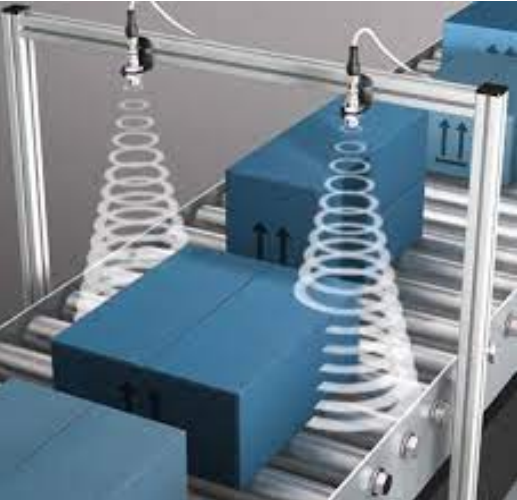
\includegraphics[width=0.4\textwidth]{sensorultra.png}
		\caption{Sensor Ultrasónico} 
	\end{figure}
	
	\item \textbf{Sensores láser}: Un sensor láser es un dispositivo que utiliza tecnología láser para medir distancias, detectar objetos o mapear entornos. Funciona emitiendo un haz de luz láser que se refleja en los
	objetos cercanos y regresa al sensor, lo que permite calcular la distancia entre el sensor y el
	objeto mediante el tiempo que tarda la luz en regresar. Los sensores láser son ampliamente
	utilizados en aplicaciones como la navegación autónoma de robots, mapeo en 3D,
	detección de obstáculos y sistemas de localización. Su alta precisión y capacidad para
	operar en entornos complejos los hacen esenciales en la robótica avanzada, especialmente
	en robots móviles y vehículos autónomos.
	\begin{figure}[H]
		\centering
		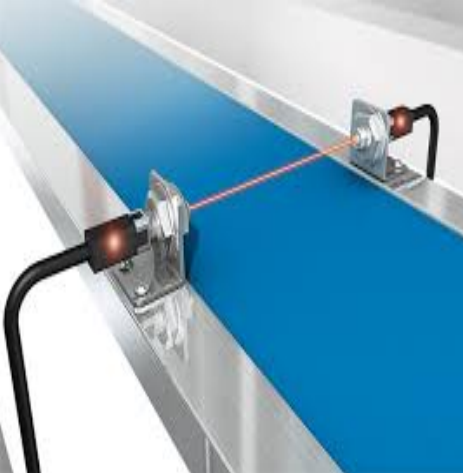
\includegraphics[width=0.4\textwidth]{sensorlaser.png}
		\caption{Sensor láser} 
	\end{figure}
	
	Los láseres son ampliamente utilizados en robótica, especialmente en sensores de
	medición láser. Su implementación permite a los robots lograr un posicionamiento, control y
	detección de seguridad de alta precisión, lo que contribuye significativamente a mejorar la
	productividad y la calidad del producto
	
	
	\item \textbf{Sensores de visión}: Un sensor de visión es un dispositivo tecnológico utilizado para capturar imágenes y procesarlas, con el objetivo de interpretar información visual en el entorno de un sistema o
	robot. Estos sensores funcionan mediante cámaras o sistemas ópticos avanzados que
	analizan imágenes y extraen datos relevantes, como la forma, el color, la posición o el
	movimiento de los objetos en su campo de visión. Son fundamentales para tareas como la
	inspección, la detección de fallos, la navegación autónoma y la manipulación precisa de
	objetos, mejorando la flexibilidad, precisión y eficiencia en sistemas automatizados y robots.
	\begin{figure}[H]
		\centering
		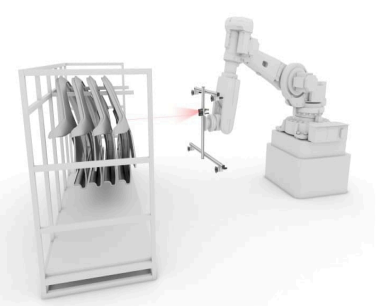
\includegraphics[width=0.4\textwidth]{sensordevis.png}
		\caption{Sensor de visión} 
	\end{figure}
	
	Los sensores de visión están diseñados para adaptarse a diversas variaciones ambientales,
	permitiendo su uso en celdas preconfiguradas sin la necesidad de ajustes costosos. Entre
	sus funcionalidades destacan el aumento de la flexibilidad, la posibilidad de ejecutar
	múltiples tipos de inspección en una sola imagen, la generación de datos detallados para
	mejorar la calidad y los procesos, y la capacidad de ajustarse a desalineaciones en el
	manejo de objetos. Entre sus principales beneficios se incluye la identificación de
	características difíciles de detectar por otros sensores, mejorando el brillo, contraste e
	iluminación de las imágenes a través de filtros y sistemas de iluminación ajustables, y
	gestionando desalineaciones e irregularidades sin importar la velocidad o posición de los
	objetos. Además, su configuración y programación son más sencillas gracias a las
	comunicaciones integradas por Ethernet, lo que facilita la comunicación de los resultados
	con otros sistemas.
	\begin{figure}[H]
		\centering
		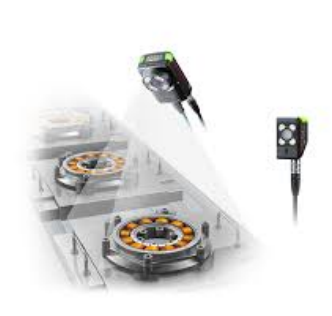
\includegraphics[width=0.4\textwidth]{sensorvision.png}
		\caption{Sensor de visión} 
	\end{figure}
\end{itemize}
\section{\textbf{Giroscopio}} 
Un giroscopio es un dispositivo utilizado para medir o mantener la orientación y la velocidad angular de un objeto. Su principio de funcionamiento se basa en la conservación del momento angular, lo que le permite detectar cambios en la orientación sin depender de referencias externas. Se emplea en diversas aplicaciones, incluyendo sistemas de navegación inercial, estabilización de vehículos y tecnología aeroespacial.
\subsection{\textbf{Tipos de Giroscopios}}
Existen varios tipos de giroscopios, cada uno con un principio de funcionamiento distinto:

\subsubsection{\textbf{Giroscopios Mecánicos}}
Son compuestos por un rotor que gira rápidamente dentro de un marco o montura.Al girar, el rotor mantiene su orientación debido a la inercia, lo que permite detectar cambios en la posición angular. Se utilizan en aplicaciones como submarinos, aviones y sistemas de estabilización.


\subsubsection{\textbf{Giroscopios Ópticos}}

No tienen partes móviles y funcionan con principios ópticos basados en interferencia de luz. Incluyen los giroscopios de fibra óptica (FOG) y los giroscopios láser de anillo (RLG). Son altamente precisos y se usan en sistemas de navegación de alta precisión, como aeronaves y satélites.


\subsubsection{\textbf{Giroscopios MEMS (Sistemas Microelectromecánicos)}}

Son dispositivos miniaturizados que utilizan la vibración de estructuras internas para detectar cambios en la orientación. Estos s encuentran en teléfonos móviles, drones y dispositivos electrónicos portátiles debido a su pequeño tamaño, bajo costo y eficiencia.


\subsection{\textbf{Funcionamiento del Giroscopio}}
El principio fundamental del giroscopio es la conservación del momento angular, lo que significa que un objeto en rotación mantiene su orientación a menos que una fuerza externa actúe sobre él. Cuando se intenta cambiar la dirección del eje de rotación, el giroscopio responde con un fenómeno llamado precesión, moviéndose en un eje perpendicular a la fuerza aplicada.

En términos matemáticos, la velocidad de precesión se expresa como:

\begin{equation}
	\omega_p = \frac{\tau}{L}
\end{equation}

donde:
\begin{itemize}
	\item $\omega_p$ es la velocidad de precesión,
	\item $\tau$ es el torque aplicado,
	\item $L$ es el momento angular del sistema.
\end{itemize}

En términos prácticos, los giroscopios pueden medir la velocidad angular al detectar la desviación de su rotor o elementos internos con respecto a su posición inicial. En los sistemas ópticos y MEMS, esta medición se realiza mediante sensores electrónicos que convierten las variaciones en señales eléctricas para su procesamiento.

\subsection{\textbf{Aplicaciones del Giroscopio}}
Los giroscopios tienen una amplia gama de aplicaciones en diferentes industrias:

\begin{itemize}
	\item \textbf{Navegación inercial:} En aviones, barcos y submarinos, los giroscopios permiten mantener la orientación sin depender de señales externas como el GPS.
	\item \textbf{Tecnología aeroespacial:} Se emplean en satélites y naves espaciales para el control de actitud y estabilización.
	\item \textbf{Electrónica de consumo:} Se encuentran en teléfonos inteligentes, consolas de videojuegos y cámaras para detectar movimientos y mejorar la experiencia del usuario.
	\item \textbf{Vehículos autónomos y drones:} Ayudan a mantener la estabilidad y orientación durante el movimiento.
\end{itemize}
\begin{figure}[H]
	\centering
	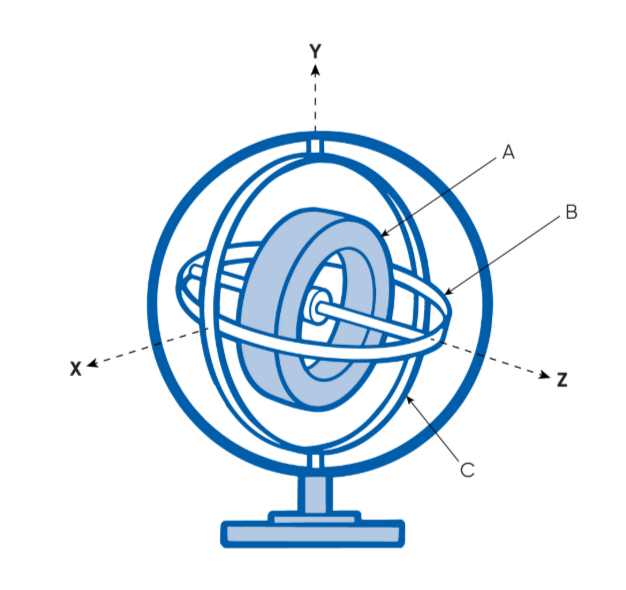
\includegraphics[width=0.35\textwidth]{giroscopio.png}
	\caption{Giroscopio}
\end{figure}
\input{secciones/Acelerómetro}
\input{secciones/Magnetómetro}
	\section{\textbf{LiDAR}} El LiDAR (acrónimo de Light Detection and Ranging) es una tecnología de teledetección que utiliza pulsos de luz láser para medir distancias y movimientos precisos en un entorno en tiempo real. Esta técnica permite generar mapas topográficos detallados y modelos 3D de alta precisión, siendo esencial en aplicaciones como la navegación de vehículos autónomos y la evaluación de riesgos naturales.
\subsection{\textbf{¿Cómo funciona LiDAR?}}
El sistema LiDAR funciona midiendo el tiempo que tarda un pulso de luz láser en viajar desde el sensor hasta un objeto y regresar. Dado que la velocidad de la luz es constante, este tiempo de recorrido permite calcular la distancia con gran precisión.

\subsubsection{\textbf{Componentes Principales}}
\begin{itemize}
	\item \textbf{Escáner láser}: Emite pulsos de luz infrarroja.
	\item \textbf{Sensor LiDAR}: Recoge los pulsos reflejados en los objetos del entorno.
	\item \textbf{Procesador}: Calcula la distancia basada en el tiempo de retorno del pulso y genera una nube de puntos tridimensional.
\end{itemize}

El proceso se repite millones de veces por segundo, generando un mapa tridimensional detallado del entorno. Estos datos pueden ser usados en simulaciones, sistemas de navegación y modelado del terreno.
\subsection{\textbf{¿Para qué sirve LiDAR?}}
El LiDAR tiene una amplia gama de aplicaciones en diversas industrias:

\subsubsection{\textbf{Agricultura}}
\begin{itemize}
	\item Mide la topografía de los terrenos agrícolas.
	\item Permite estimar la biomasa de los cultivos y detectar propiedades del suelo.
\end{itemize}

\subsubsection{\textbf{Aeroespacial y Defensa}}
\begin{itemize}
	\item Se usa para mapear terrenos con alta precisión.
	\item Rastrea objetivos y apoya la planificación de misiones militares.
\end{itemize}

\subsubsection{\textbf{Automoción}}
\begin{itemize}
	\item Es clave en la navegación de vehículos autónomos.
	\item Mejora la seguridad mediante la detección y análisis del entorno en tiempo real.
\end{itemize}

\subsubsection{\textbf{Silvicultura}}
\begin{itemize}
	\item Permite mapear el dosel forestal con gran detalle.
	\item Ayuda en la gestión y conservación de recursos forestales.
\end{itemize}

\subsubsection{\textbf{Geología y Minería}}
\begin{itemize}
	\item Se usa para la cartografía de minas y yacimientos.
	\item Optimiza la planificación de operaciones mineras.
\end{itemize}
\begin{figure}[H]
	\centering
	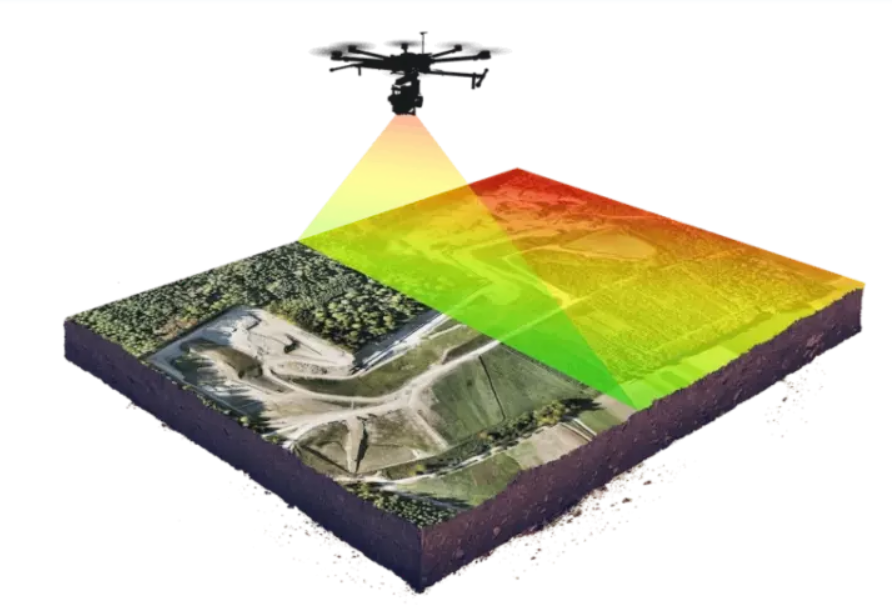
\includegraphics[width=0.35\textwidth]{lidar.png}
	\caption{LiDAR}
\end{figure}

\section{\textbf{Conclusión}} Los sensores son herramientas esenciales para que los robots y otros dispositivos puedan percibir y reaccionar a su entorno. En este reporte, se exploraron distintos tipos de sensores, tanto internos como externos, que ayudan a medir posición, velocidad, aceleración y fuerza. También se analizaron sensores más avanzados, como los giroscopios, acelerómetros, magnetómetros y el sistema LiDAR.

Cada sensor tiene una función importante. Los sensores de movimiento aseguran que los robots se desplacen con precisión, mientras que los de aceleración y fuerza ayudan a mejorar la estabilidad y seguridad. Por otro lado, sensores como el giroscopio, el magnetómetro y el LiDAR permiten a los robots y vehículos autónomos ubicarse y moverse en su entorno con mayor exactitud.

Gracias a estos avances, los sensores se han convertido en una parte clave de muchas industrias, como la robótica, la exploración espacial, la seguridad y el transporte. Su continuo desarrollo permite mejorar la tecnología y facilitar tareas en nuestra vida diaria. En el futuro, seguirán evolucionando y ayudando a crear sistemas más inteligentes y eficientes.

%-------------------------------------------
% Bibliografía
%-------------------------------------------
\nocite{*}
\bibliographystyle{IEEEtran}  % Estilo de bibliografía IEEE
% La bibliografía se tomará del archivo "fuentes.bib"
\bibliography{fuentes}
	
\end{document}
